\newpage

\section{\label{MARS} MARS: A Multiple Autonomous Robot Simulator}
\markright{\arabic{section}. MARS}
\hfill {\Large \em (Preliminary Announcement)}

\hfill {\em Author: Yasuo KUNIYOSHI, ETL}

{\bf MARS} is a graphical simulation environment for multiple autonomous
mobile robots in 2D space.  This program is written in EusLisp.

{\bf Development Status:} As of Janurary, 1995, a pre-release version
of MARS is in use within ETL. We are actively improving the system and
plan to release the first version within the first half of 1995. We
will continue enhancing the system thereafter and hopefully achieve a
stable state by March 1996. Release announcements will be made through
the euslisp mailing list and other internet services.
Possibly we will adopt licencing conditions separate from the EusLisp.

{\bf Purpose:}
MARS is intended for use in intelligent robotics research on
single/multiple mobile robot(s), such as behaviour learning, map
building, collective intelligence, multi-robot cooperation,
cooperative learning, etc.


\subsection{How to Start} The MARS program resides in {\bf
robot/MARS/ver.XXX}. First, copy the ".eursrc" file to your home
directory. Make necessary changes. (Pathname of the directory in which
MARS is installed.)

Invoke {\bf eusx} in this directory,  and all the files are
automatically loaded and the simulator starts running.
Wait until a window opens and an initial message appears in the bottom window.

Example:
\begin{verbatim}
Try "SYSTEM"->"Load" menu.
Load "example.bbs".
And "SCL"->"On" menu.
\end{verbatim}

Notes:\\
SCL$\rightarrow$"Off" Pauses the simulation but continue GUI processing.\\
SYSTEM$\rightarrow$"Quit" Exits the toplevel loop. Can be resumed by (mars-loop).\\
SYSTEM$\rightarrow$"Save" Saves the current state to a file.\\
SYSTEM$\rightarrow$"All-Clear" Clears everything and initializes the system.\\
SYSTEM$\rightarrow$"Reset" Is used to reset internal states of the robots
(Special purpose).\\

\subsection{System Overview}

\begin{figure}[h]
\begin{center}
%\begin{tabular}{c@\extracolsep{1em}c}
\begin{tabular}{c c}
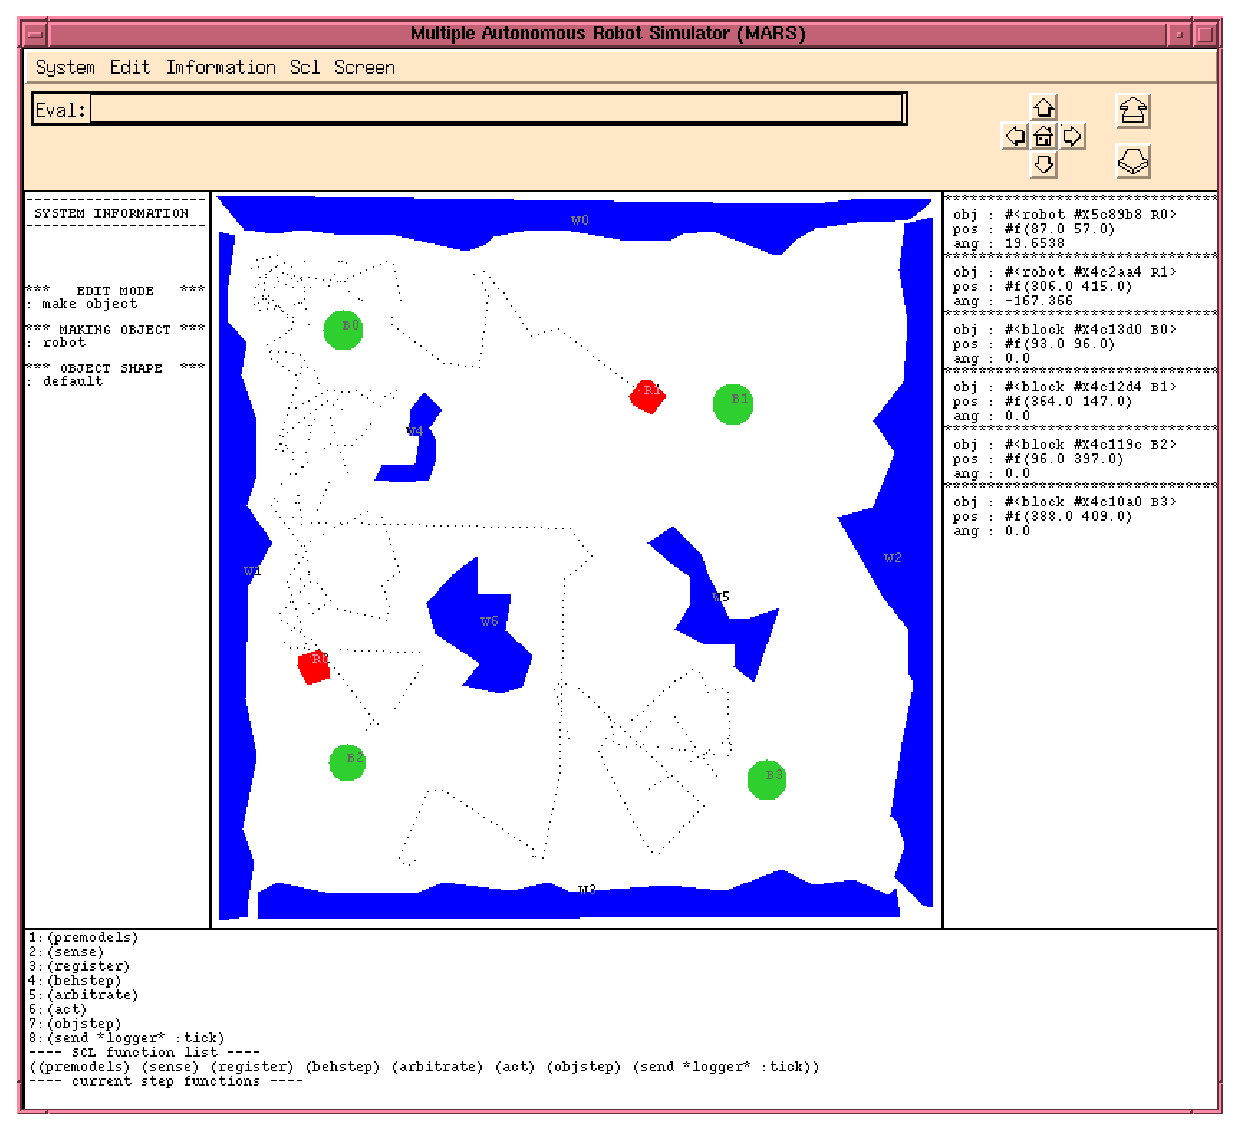
\includegraphics[height=10cm]{fig/mars.ps}
%\epsfile{file=fig/mars.eps,scale=0.3} & % ɽ���Ʊ�������ѹ����ơ�
%\mbox{
%\epsfsize=10cm
%\epsfbox{file=fig/mars.eps}
%}
%\epsfile{file=fig/simst.ps,hscale=0.42,vscale=0.45} \\
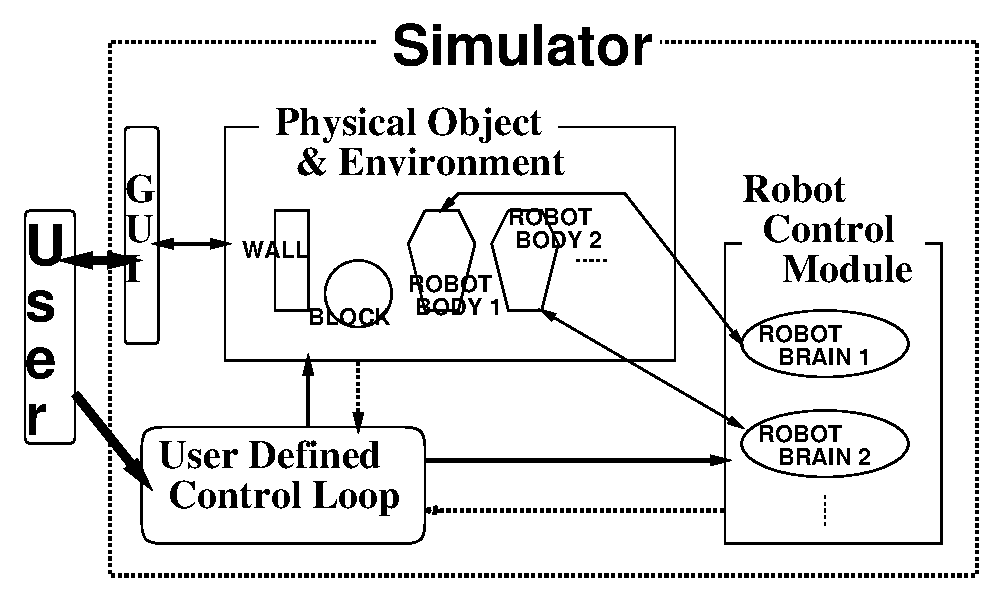
\includegraphics[height=10cm]{fig/simst.ps}
%\mbox{
%\epsfsize=10cm
%\epsfbox{file=fig/simst.ps}
%}
\end{tabular}
\caption{\label{MARSOverview} MARS window display example (left).
And overall program structure (right).}
\end{center}
\end{figure}

When you start up MARS, you will see the main window as shown in
Fig.~\ref{MARSOverview}(left). The MARS system adopts a modular
architecture as in Fig.~\ref{MARSOverview}(right). It consists of
a physcial simulation module, robot control modules, a graphical user
interface module (GUI), and a user defined global control loop.

{\bf Physical Simulation:}
Our current physical simulation module handles four types of objects,
{\bf wall} (static obstacles), {\bf block} (passive objects), {\bf
robot-body} (active objects), and {\bf magic-block} (special
reward-giving objects for learning experiments).

\begin{figure}
\begin{center}
%\begin{tabular}{c@\extracolsep{1em}c}
\begin{tabular}{c c}
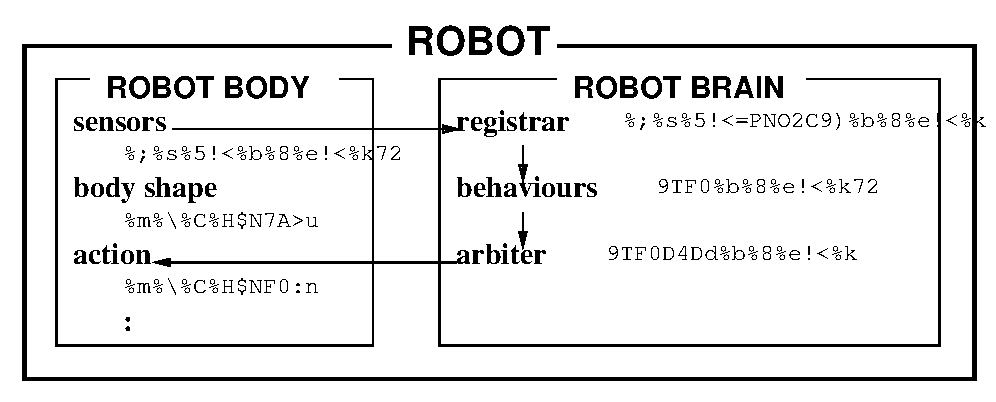
\includegraphics[width=10cm]{fig/robot-ui2.ps}
%\epsfile{file=fig/robot-ui2.ps,hscale=0.5,vscale=0.5} &
%\mbox{
%\epsfsize=10cm
%\epsfbox{file=fig/robot-ui2.ps}
%}
%\epsfile{file=fig/robot-st2.ps,scale=0.4} \\
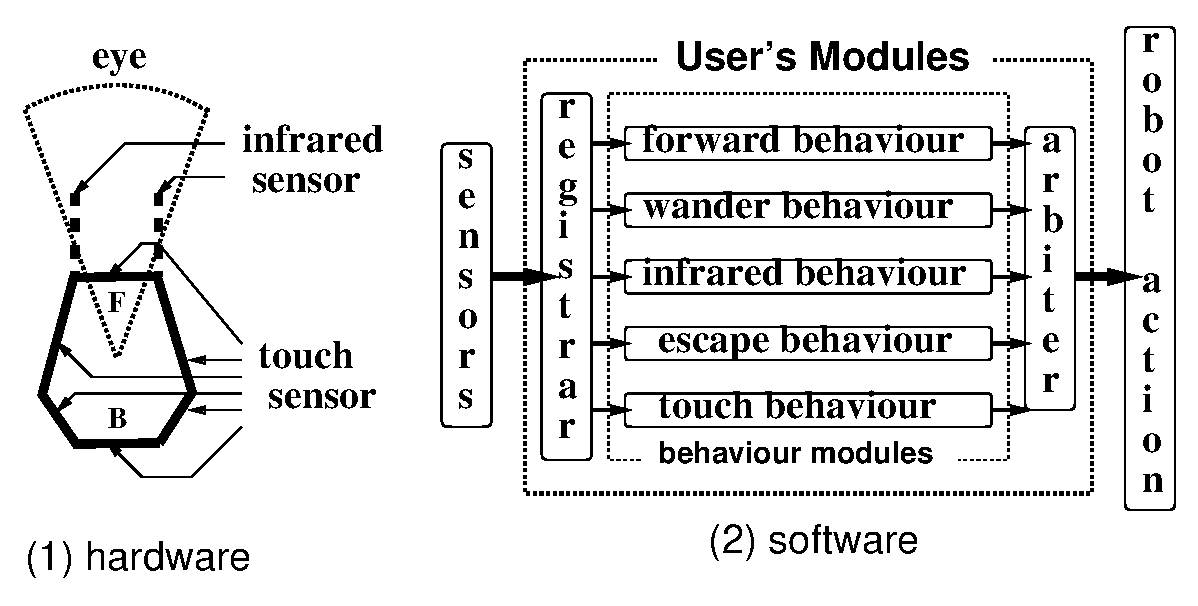
\includegraphics[width=10cm]{fig/robot-st2.ps}
%\mbox{
%\epsfsize=10cm
%\epsfbox{file=fig/robot-st2.ps}
%}
\end{tabular}
\end{center}
\caption{\label{fig:robotst} Internal structure of a robot object
(left). And an example behavior-based robot configuration (right).}
\end{figure}

{\bf Robot Models:}
There is a clear interface between the physical simulation module and
robot control modules. Any number of {\bf robot} models can be
generated and simulated in (pseudo-)parallel.
Each {\bf robot} consists of a pair of modules,
a {\bf robot-body} and a {\bf robot-brain}.
A {\bf robot-body} defines physical properties of a robot and a {\bf
robot-brain} defines how the robot behaves.

{\bf Sensor Models:}
A user can choose and attach any number of sensors to any place of a
{\bf robot-body}. Currently available sensor models are as follows:
{\bf distance} (odometry), {\bf angle} (rotation), {\bf touch}, {\bf
infrared}, {\bf radar} (sonar), {\bf eye} (object-name-sensor).
Noise or uncertainty is not considered in the current version.

{\bf Robot Brains:}
A {\bf robot-brain} is a user defined module for processing the
simulated sensor data and generating action commands.
It must accept sensor data and output action commands. In addition, it
must be written as a re-entrant program, time-sliced by a {\bf :step}
message sent by the global control loop.
As long as these constraints are met, a user can adopt any cognitive
architecture. The system provides an example behavior-based type
architecture as a default.

{\bf GUI:}
The {\bf MARS} main window has a menu-bar with several buttons for
controlling the system. Also, the system has a built-in graphical
editor for creating/modifying the physical environment.
You can save/load a physical environment definition together with
agent definitions to/from a file.

{\bf Network Extension:}
A {\bf robot-brain} can be configured to be connected to external
process via an asychronous socket connection. In this case, a user can
use an arbitrary language (C, Prolog, Scheme, Perl, etc...) to write
the {\bf remote-brain}. Thanks to the asynchronous connection, a user
do not have to mind about time slicing at all.

{\bf Facility for Learning Experiments:}
{\bf MARS} provides several special functionalities for robot learning
experiments: reward-giving objects, reward sensors (send reward values
to each robot), and a reward-logger (accumulates a system-wide reward
statistics.)

